\chapter*{Opis teoretyczny algorytmu ewolucyjnego}
Proces uczenia sygnalizacji świetlnej w tej pracy został zrealizowany z pomocą algorytmu ewolucyjnego. Ten rozdział opisuje kolejne kroki, z których składa się proces uczenia. Szczegóły dotyczące zastosowania poniższego algorytmu zostały opisane w następnym rozdziale.
\section*{Pierwsze pokolenie}
Przebieg uczenia rozpoczyna się od wygenerowania pierwszego pokolenia osobników. Osobnik to właściwie zbiór wartości określonych parametrów. W pierwszym pokoleniu wartości te generowane są losowo z zakresu określonego w konfiguracji algorytmu. 
\section*{Funkcja dostosowania}
Osobniki wygenerowanego pokolenia poddawane są ocenie, która określa ich dostosowanie (ang. \textit{fitness}). Funkcja dostosowania określona jest wzorem:
\begin{equation}
f(x) = max(t(1),\ldots, t(n)) - t(x)
\label{fitness}
\end{equation} 
gdzie:\\
\begin{tabularx}{\textwidth}{ r c l }
$x$ & -- & oceniany osobnik\\
$n$ & -- & liczba osobników w pokoleniu\\
$t(a)$ & -- & czas, w jakim określona liczba samochodów przejechała przez skrzyżowanie,\\ &&przy sygnalizacji ustawionej wg parametrów osobnika $ a $
\end{tabularx}
\section*{Generowanie nowego pokolenia}
Najlepszy osobnik poprzedniego pokolenia jest kopiowany wprost do nowego. 
Wybór reszty osobników odbywa się drogą selekcji turniejowej. Z poprzedniego pokolenia losowane są 3 osobniki. Spośród tych trzech wybierany jest ten o najwyższej wartości funkcji dostosowania. Taki turniej powtarzany jest $2n$ razy, gdzie $n$ to liczba osobników w pokoleniu (określona w konfiguracji algorytmu). Następnie ze zbioru $2n$ osobników wybieranych jest $n$ o najlepszej wartości funkcji dostosowania. Ta pula poddana jest następnie krzyżowaniu lub mutacji.
\section*{Mutacja i krzyżowanie}
Każdy osobnik z wygenerowanej puli, z wyjątkiem najlepszego zachowanego z poprzedniego pokolenia, zostaje zmutowany albo skrzyżowany z innym osobnikiem. Decyduje o tym ważone losowanie. Prawdopodobieństwo, że osobnik zostanie poddany mutacji jest zmienne i wyznacza je funkcja:
\begin{equation}
f(x) = (sin(x * \frac{1}{\frac{g}{1000}+\frac{x}{100}})+1) : 2 \cdot m
\label{mutRate}
\end{equation}
gdzie:\\
\begin{tabularx}{\textwidth}{ r c l }
	$x$ & -- & numer obecnego pokolenia\\
	$g$ & -- & liczba wszystkich pokoleń, określona w konfiguracji algorytmu\\
	$m$ & -- & maksymalny współczynnik mutacji, określony w konfiguracji algorytmu\\
	&&\\
\end{tabularx}\\
Wykres tej funkcji przedstawiono na rysunku~\ref{fig:mutRate}.\\
Korzyści wynikające ze stosowania dynamicznego współczynnika mutacji opisał Thierens~\cite{EvolutionaryComputation2002}. Również przy powstawaniu tej pracy zmienne prawdopodobieństwo mutacji okazało się lepszym rozwiązaniem w porównaniu do stałego współczynnika.

\begin{figure}[h]	
	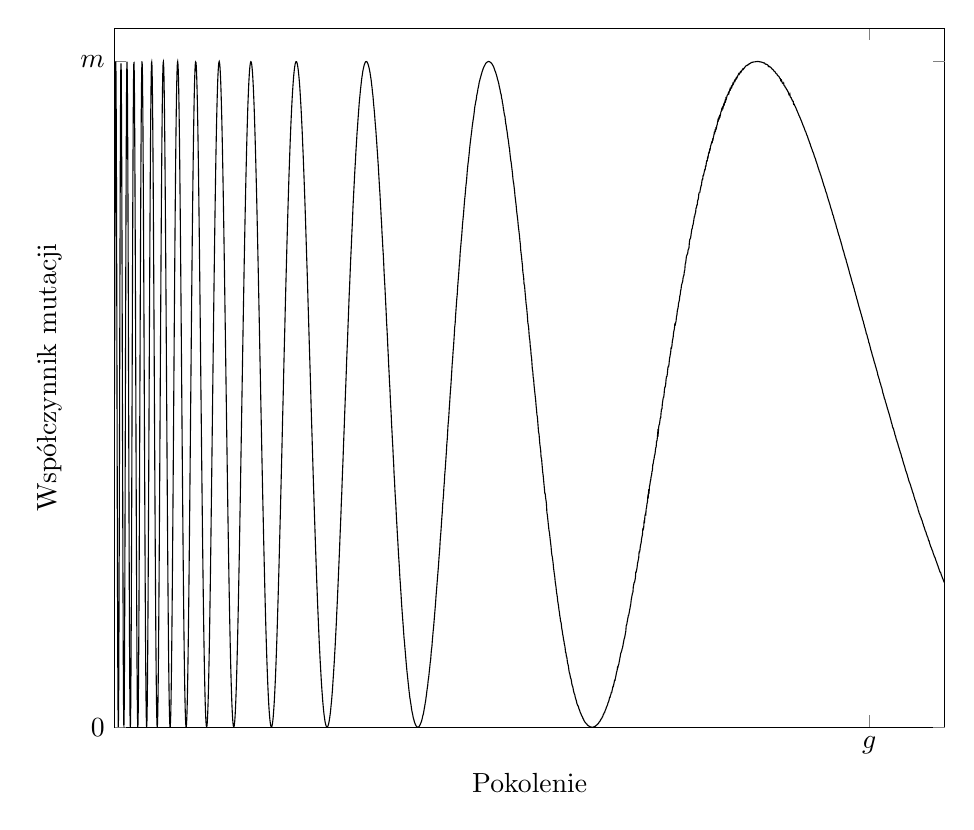
\begin{tikzpicture}
	\begin{axis}
	[
	domain=0:110,
	width=\textwidth,
	xlabel=Pokolenie,
	ylabel=Współczynnik mutacji,
	xmin=0,
	xmax=110,
	ymin=0,
	ymax=1.05,
	samples=2000,
	xtick=100,
	xticklabel={$g$},
	ytick={\empty},
	extra y ticks={0,1},
	extra y tick labels={0,$m$},
	smooth
	]
	\addplot+[mark=none, black]{(sin(x * (1 / (0.1 + (x / 100.0)))*(180/3.14)) + 1.0)/2.0};
	\end{axis}
	\end{tikzpicture}
	\caption{Funkcja określająca współczynnik mutacji}
	\label{fig:mutRate}
\end{figure}
\pagebreak
Mutacja polega na losowym dodaniu lub odjęciu od wartości każdego parametru osobnika losowej liczby z zakresu 1--20. \\
Jeśli w wyniku wyżej opisanego losowania zostanie podjęta decyzja, że osobnik ma zostać poddany krzyżowaniu, to z puli losowo wybierany jest inny osobnik, od którego ten pierwszy przejmie wartość co drugiego parametru. Pozostałe parametry pozostają bez zmian.

Po zastosowaniu krzyżowania lub mutacji nowe pokolenie jest gotowe do oceny funkcją dostosowania opisaną wcześniej, co zamyka cykl. Kolejne pokolenia są generowane na postawie poprzednich i oceniane tak długo, aż osiągnięta zostanie liczba pokoleń określona w konfiguracji algorytmu.